\section{课题来源及研究的目	的和意义}
\subsection{课题来源}
核技术被越来越多地应用于生产生活的各个领域,发挥越来越重要的作用。
在世界应对气候变化的严峻挑战和不断加剧的能源紧张问题下,核能也作为一
种不可或缺的清洁能源迅猛发展,
为未来的能源发展提供选择。核技术的发展于人们的生活密切相关,工业探伤、
灭菌消毒、辐照加工、医学诊断与治疗、
空间探测、成影技术等都极大地推动着人类社会的进步
\cite{2002原子核物理}。
核技术核工程的迅猛发展
虽然促进了人类的进步,但人们受到核辐射损伤的风险也大大提高.
  
随着科学的发展,电离辐射对人体的危害
也逐渐为人们所熟知。电离辐射对人体的危害主要可分为直接作用和间接作用两类。
直接作用是指当射线直接击中生物大分子,辐射能量直接沉积在受作用的分子上,
引起其激发和电离,
使生物大分子化学键断裂、降解或解聚,使某些酶分子活性降低或失活,从而导致细
胞正常功能和代谢
发生障碍或受到干扰
;间接作用是指辐射引起机体中水分子的电离和激发,成簇产生的原发电离产物
如$ \mathrm{H_2O_2} $、 $ \cdot \mathrm{H} $ 、$ \cdot \mathrm{OH} $ 、
$ \mathrm{H}^+ $ 、 $ \mathrm{OH}^- $  
等,对生物活性大分子造成损伤。根据机体受照射剂量的不同,会出现白内障、
皮肤良性损伤等确定性效应和以癌症为主的随机性效应。
由于电离辐射可以造成严重的辐射损伤,因此我们有必要研究其屏蔽防护
,以便寻找出合适的屏蔽物质来保护人体。
\cite{霍雷2015辐射剂量与防护}


在航空航天领域,高能射线除了会对人体造成损伤外,空间辐射环境对航天器的辐
射损伤机制主要为电离和位移。 电离是指入射粒子
诱发材料中靶原子的电离,进而形成电子空穴对。电离可以引起器件性能退化,产生单粒
子效应、总剂量效应等\cite{slayman2011jedec,8892478}。 位移是指入射
粒子与材料原子相互作用并产生动能交换,进而靶
原子离开原来位置并形成间隙原子和空位。位移产生的间隙原子或空位一般具有较强的活
性,是半导体材料或器件中的载流子源,或者是载流子的俘获陷阱。 由于以上作用机制,
在深空环境中,高能宇宙射线会诱发航天器产生永久性故障或暂时
性损伤。因此,寻求一种合适的材料来保护航天器是深空探索中不可或缺的一
环\cite{沈自才2020航天器空间辐射防护材料与防护结构}。
\begin{figure}[h]
    \centering
    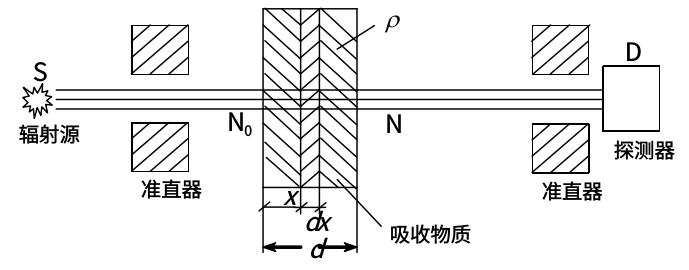
\includegraphics[width = 0.6\textwidth]{图片1.png}
    \caption{获得单能窄束$ \gamma $ 射线示意图}
    \end{figure}
    
$ \gamma $辐射是高能光子射线,具有较强的穿透能力,与物质发生的相
互作用主要包括康普顿效应、
光电效应和电子对效应三种物理过程。
在已发现的上千种放射性核素中,大部分都能放射出$ \gamma $射线,
$\gamma$射线的应用也很广泛,经常需要对$\gamma$射线进行防护,
确保机体健康和工业装置正常运行,
因此,对$\gamma$射线的防护相当重要。

对于单能窄束的$ \gamma $射线,
即平行入射的单一能量的
$ \gamma $ 射线,
假设屏蔽物质的厚度为$ d $ ,密度为$ \rho $ ,
穿过吸收物质前的强度为$I_0$,穿过吸收物质后的强度为$I$
其在物质中的衰减规律满足\eqref{ib}式。单能窄束$ \gamma $ 射线
可如图1方式获得,这里的窄束指的是物理意义上的窄束,即射线束可以有一定
的宽度,但其中没有
被散射的光子。
    \begin{equation}
        I=I_0\mathrm{e}^{-\mu d}  \label{ib}
    \end{equation}
其中系数$\mu$线衰减系数。

对于未经准直的宽束的入射$\gamma$射线,在探测器和放射源与有准直
的$\gamma$射线示意图入射
相同时,由于探测器接收到的$\gamma$射线不仅包括未与物质相互作
用的$\gamma$射线,
还有经过相互作用改变原来方向的散射$\gamma$射线,因此
探测器的计数强度比窄束情况高很多,如图2:
\begin{figure}[h]
    \centering
    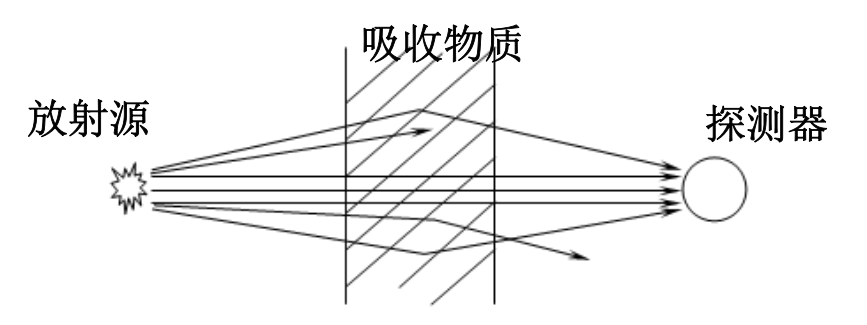
\includegraphics[width = 0.6\textwidth]{图片2.png}
    \caption{未经准直的宽束$ \gamma $ 射线经过物质的减弱示意图}
    \end{figure}

此时$\gamma$射线的减弱规律可表示为
\begin{equation}
    I=I_0B\mathrm{e}^{-\mu d}  \label{i}
\end{equation}
式中$B$为累积因子,用于描述因散射改变方向而被探测器接受到的$\gamma$射
线\cite{霍雷2015辐射剂量与防护}。

基于以上分析, 本课题将重点研究$\gamma$射线与物质相互作用过程中累积因子的规律。
在前期文献调研的
基础上,我们发现: 在研究大量粒子与物质的相互作用时,理论与实验都难以进行详细讨
论。原因在于理论只能处理单个粒子或多个粒子(并非大量)在物质中的运动规律,实验
不能详细地统计每个光子的散射偏转,且实验材料等条件会严重受到成本因素的制约
,而模拟计算可以很好的解决以上两个问题。 由欧洲核子中心开发的蒙特卡洛程序包
Geant4 可以用来模拟多种粒子(中子、电子、质子、光
子、重带电粒子等)与物质的相互作用。仿照真实的物理实验场景,通过各种物理反应过
程截面的蒙特卡罗抽样来模拟真实的物理过程。 本课题将利用 Geant4 来模拟$\gamma$
射线屏蔽中,射线穿过屏蔽物质时发生的物理过程,可以节约实验成本,摆脱实验条件的限制。
根据模拟计算的数据得到相应的累积因子,将模拟结果与理论计算结果对照,
可对理论公式进行补充与修正。图3为利用Geant4运行一个案例流程。
\begin{figure}[h]
    \centering
    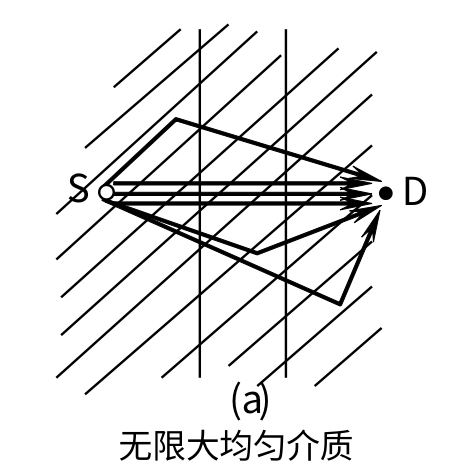
\includegraphics[width = 0.5\textwidth]{图片3.png}
    \caption{Geant4中运行一个案例的流程图}
    \end{figure}
\subsection{研究目的及意义}
目前现有的累积因子参考值为均匀无限大介质情况的累积因子数值,但在实际的屏
蔽设计中只能采用有限大
的介质进行屏蔽,由于无限大介质的累积因子显然高于有限大介质,因此虽然按照无限大介质的累积因子数值进行$\gamma$射线的屏蔽
计算可以得到较为安全的结果,但却增加了屏蔽介质的成本\cite{2008Overview}。
本课题通
过模拟$\gamma$射线在有限大介质中的衰减的物理过程,
来研究贴近现实的情况下累积因子B的规律
,进而得到对人体、仪器设备等屏蔽效果最佳的若干种方案, 并通过调整介质种类
与厚度等参数, 在可接受的防护效果下减少成本,达到防护效果与成果的平衡。 
另外, 本课题利用 Geant4 进行模拟可以
弥补理论上只能计算单个粒子,实验条件限制材料的大小、厚度以及探测距离的选择等
不足,对累积因子的理论公式进行补充,使其可以更好地指导实践。

% \begin{figure}[h]
%     \centering
%     \includegraphics[width = 0.4\textwidth]{golfer}
%     \caption{打高尔夫球的人,硕士论文要求只用汉语}
%     \end{figure}
    

% \begin{figure}[htbp]
%     \centering
%     \begin{minipage}[t]{0.4\textwidth}
%     \centering
%     \includegraphics[width=\textwidth,height=\textwidth]{golfer}
%     \caption{打高尔夫球的人。注意,此图对齐方式是图片底部对齐}
%     \end{minipage}
%     \centering
%     \begin{minipage}[t]{0.4\textwidth}
%     \centering
%     \includegraphics[width=\textwidth]{golfer}
%     \caption[golfer6]{}{打高尔夫球的人}
%     \end{minipage}
%     \end{figure}

% \begin{table}[htbp]
%     \caption{符合研究生院绘图规范的表格}
%     \vspace{0.5em}\centering\wuhao
%     \begin{tabular}{ccccc}
%     \toprule[1.5pt]
%     $D$(in) & $P_u$(lbs) & $u_u$(in) & $\beta$ & $G_f$(psi.in)\\
%     \midrule[1pt]
%      5 & 269.8 & 0.000674 & 1.79 & 0.04089\\
%     10 & 421.0 & 0.001035 & 3.59 & 0.04089\\
%     20 & 640.2 & 0.001565 & 7.18 & 0.04089\\
%     \bottomrule[1.5pt]
%     \end{tabular}
%     \end{table}
\section{国内外在该方向的研究现状及分析}
国内研究者在前十几年已经开始利用蒙特卡洛方法对一些物理过程进行模
拟计算。王军成等用 MCNP4C 程序模拟了 $\gamma$ 射线经铅
等材料在
有准直器及无准直器情况下屏蔽后剂量率随这些屏蔽材料的厚度的变化关系,
MCNP是由美国的洛斯阿拉莫斯实验室研制出来的大型多功能蒙特卡罗计算程序,
能够计算复杂结构中的中子、光子、电子及它们的耦合输运问题,
γ 射线穿过屏蔽材料的过程中,部分 γ 射线被材料吸收,
部分 γ 射线在材料中发生散射,不同的屏蔽材料对 γ 射线的吸收和散射概率不同,
计算了有无准直器剂量率随铅厚度的变化关系及剂量率随准直器宽深比的变化关系如图4、5
\cite{王军成2020MCNP}。
赵原等研究了无限大均匀平板模型对$\gamma$射线的累积因子$B_1^*$,并计算了其与
无限大均匀模型累积因子$B_0$的比值$B_1^*/B_0$随$B_0$的变化规律如图6
\cite{赵原2019不同计算模型对水中γ射线吸收剂量累积因子的影响}。
李华等基于蒙特卡罗方法MCNP对圆柱模型对于水中的$\gamma$射线
吸收剂量累积因子随介质尺寸的变化进行了研究
\cite{李华2017介质尺寸对水中γ射线吸收剂量累积因子的影响}。
\begin{figure}[htbp]
    \centering
    \begin{minipage}[t]{0.45\textwidth}
    \centering
    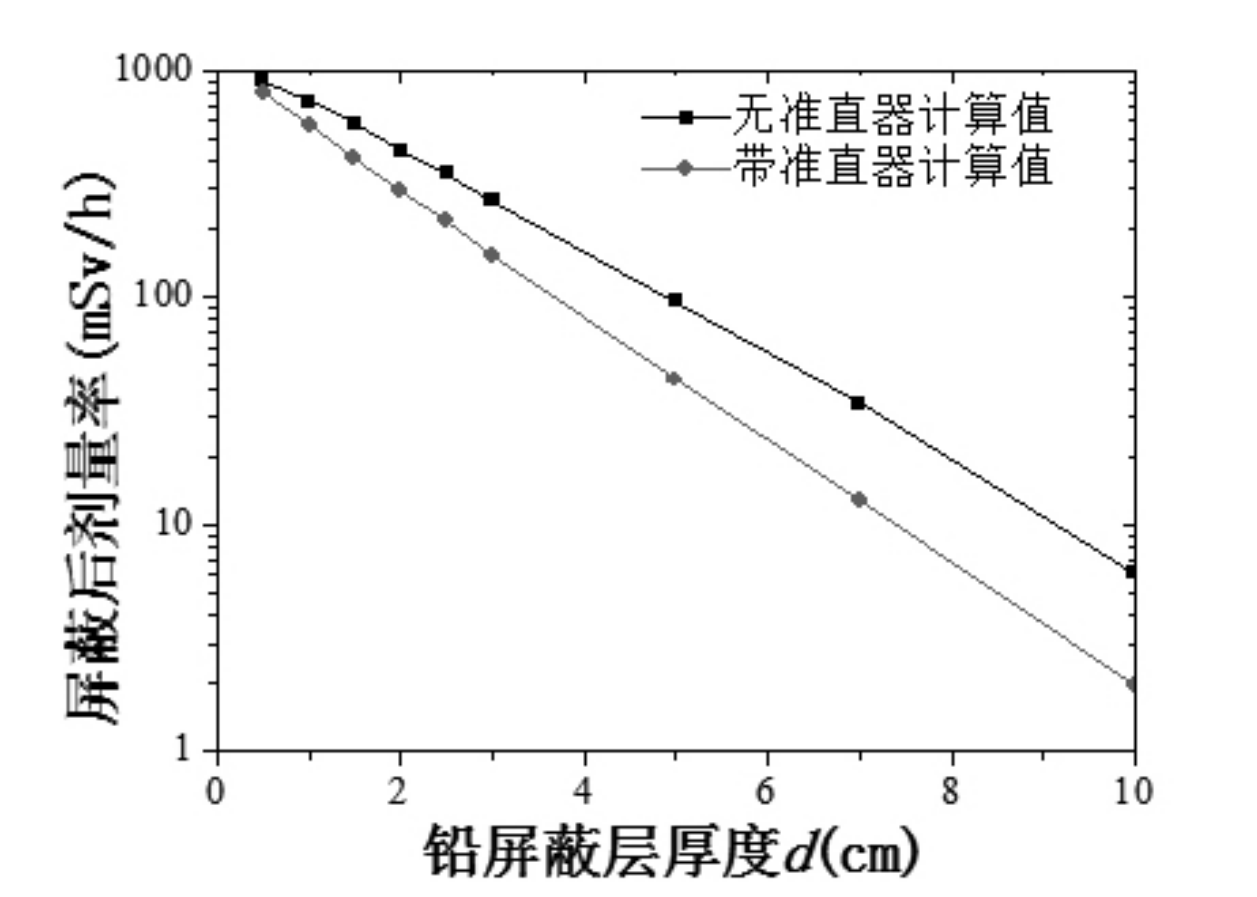
\includegraphics[width=\textwidth,height=0.71\textwidth]{Screenshot_20211117_093232.png}
    \caption{剂量率随铅厚度的变化\cite{王军成2020MCNP}}
    \end{minipage}
    \centering
    \begin{minipage}[t]{0.45\textwidth}
    \centering
    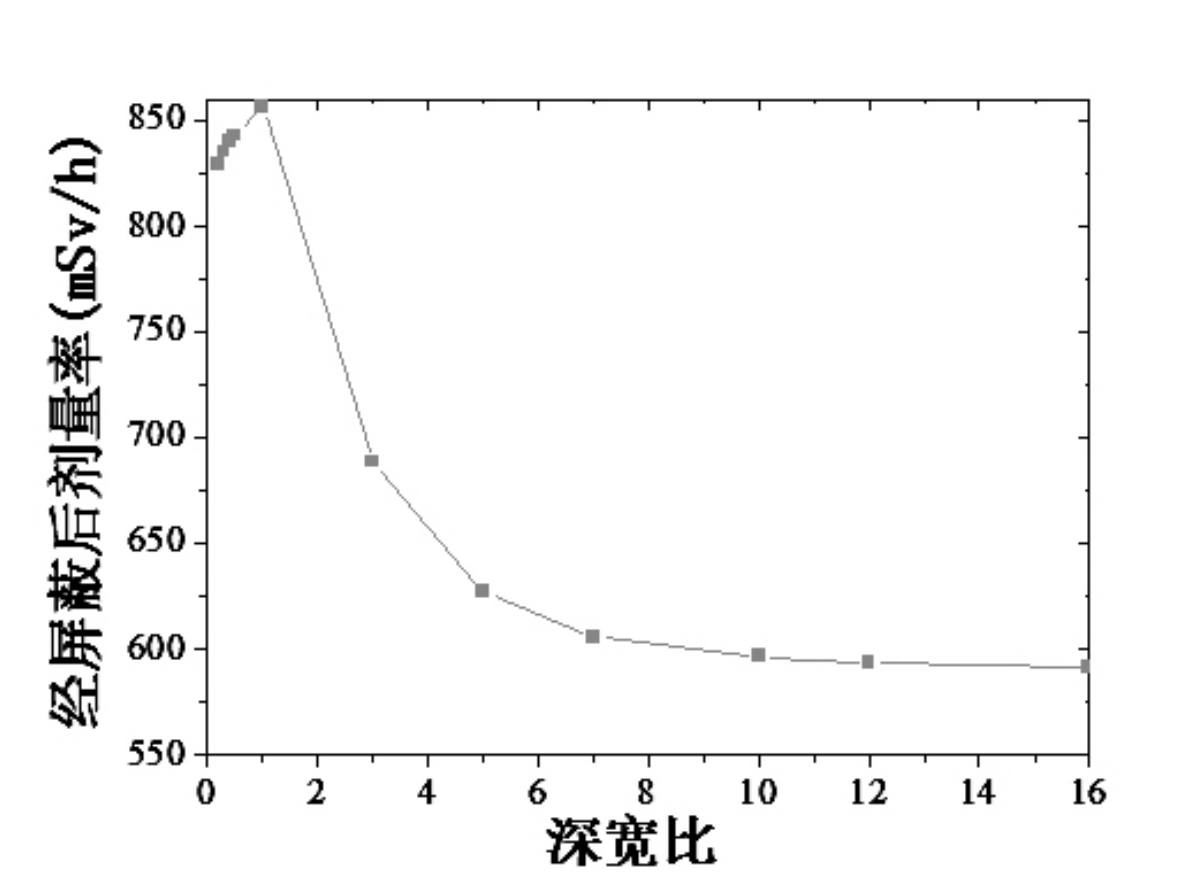
\includegraphics[width=\textwidth,height=0.73\textwidth]{Screenshot_20211117_093248.png}
    \caption{经屏蔽层屏蔽后剂量率随准直器深宽比变化的计算结果\cite{王军成2020MCNP}}
    \end{minipage}
    \end{figure}

\begin{figure}[h]
    \centering
    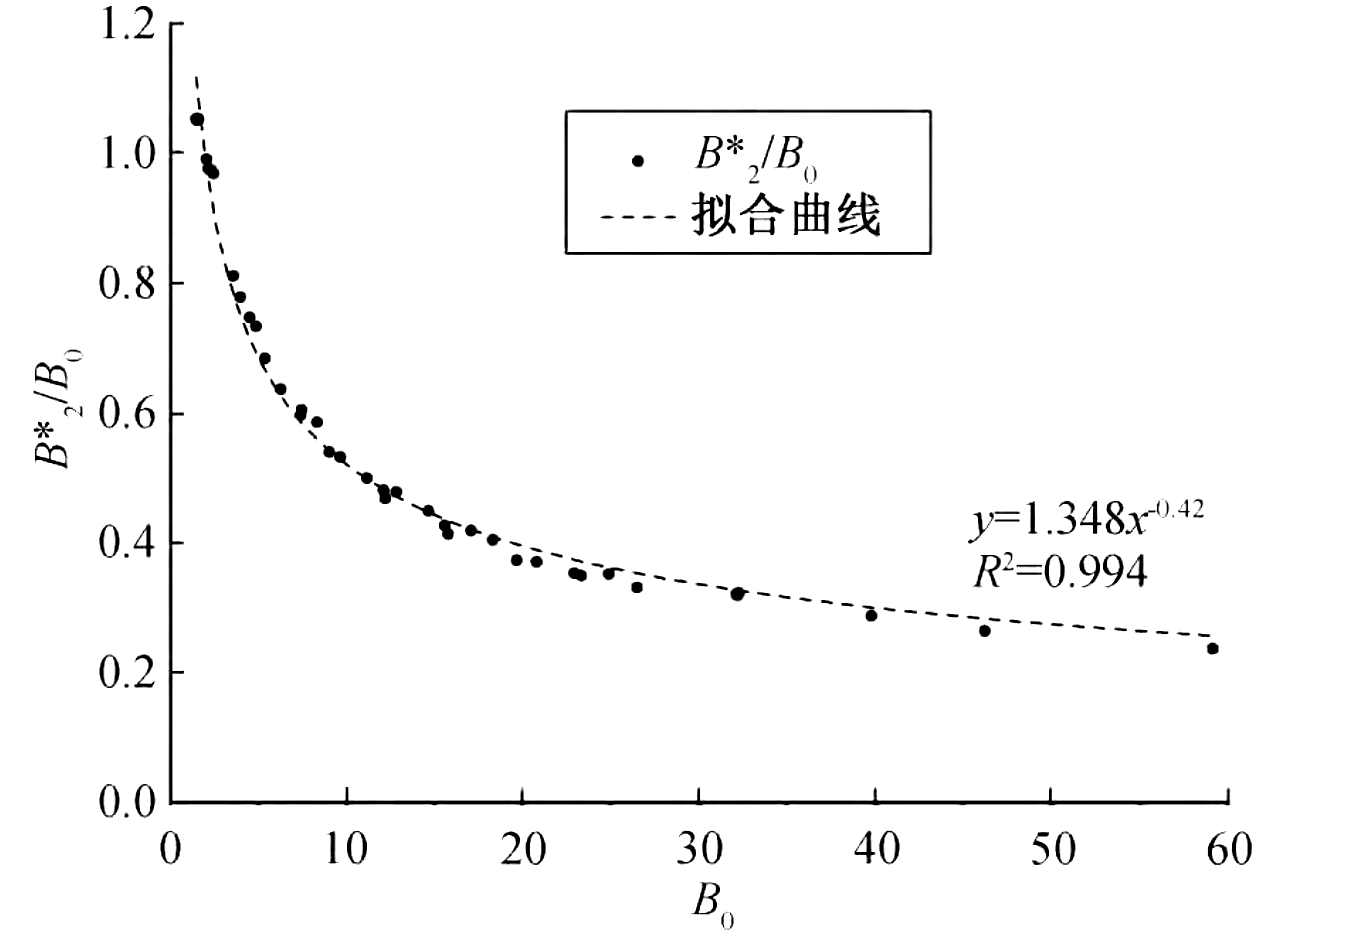
\includegraphics[width = 0.5\textwidth]{Screenshot_20211117_095417.png}
    \caption{水中$B_1^*/B_0$与$B_0$的关系曲线\cite{赵原2019不同计算模型对水中γ射线吸收剂量累积因子的影响}}
    \end{figure}

李善荣等人综述了国内外核防护材料的研究现状,
分别介绍了不同辐射的防护材料研究进展,对于$\gamma$射线,
论述了屏蔽材料针对性地以金属合金材料、高分子复合材料、
有机玻璃和混凝土等几类为主,以满足核电、放射医疗、航空电子、
辐照加工等核技术运用领域的辐射防护
\cite{李善荣2020核辐射防护材料的研究进展}。
陆宁综述介绍了不同射线的常用屏蔽材料,对于$\gamma$射线的屏蔽,
高能光子流主要产生光电效应、康普顿散射和电子对效应三种作用,
光电效应产生几率与屏蔽材料原子序数4次方成反比,
康普顿散射效应与屏蔽材料的原子序数成反比,
电子对产生与屏蔽材料原子序数平方成反比,因此
屏蔽$\gamma$射线应该选择原子序数高的元素。
\cite{陆宁2020核辐射防护服研制}
向辉云等计算了一个实际$\gamma$射线探伤室有无屏蔽情况的当量剂量率,
减弱倍数,透射比等参数,
无屏蔽和有屏蔽时$\gamma$辐射空气吸收剂量率分别满足\eqref{h1}\eqref{h2}式
\cite{向辉云0某工业γ射线探伤室的屏蔽设计与监测评价}
石勇等论述了铅材料的危害,提出用钨材料替代铅进行辐射屏蔽
\cite{石勇2019无铅复合屏蔽材料的研究}。

\begin{equation}
    \dot{H}_1=\frac{A\gamma _k}{r^2} \label{h1}
\end{equation}
\begin{equation}
    \dot{H}_2=\frac{1.45 \times 10^5A\gamma q}{r^2} \label{h2}
\end{equation}

现有的累积因子计算式为针对无限大介质模型的泰勒公式与伯杰公式。
周文明等对泰勒公式和伯杰公式计算累积因子进行比较,
在辐射屏蔽设计中,μd 在 1~20 之间时,利用伯杰公式计
算$^{137}\mathrm{Cs}$和$^{60}\mathrm{Co}$放射源的累积因子较泰勒公式小,所需屏蔽厚度较小
\cite{周文明2017两种不同经验公式法计算累积因子的比较}。
李雪琴等对直接计算法、减弱倍数法、半减弱层厚度法
三种屏蔽计算方法的结果进行比较,
结果表明半减弱层厚度法算得的结果最保守,算得剂量率最大,
对于辐照室选择防护墙厚度,从利益-代价分析来看,并不能认为越安全越好,
应遵循辐射辐射防护最优化设计的原则,合理比较三种计算结果,避免造成“防护过度”的现象
\cite{李雪琴2013辐照装置屏蔽厚度计算的方法研究与评价}。
\section{主要研究内容}
\subsection{Geant4模型与实验对比验证可靠性}
由欧洲
核子中心开发的蒙特卡洛程序包 Geant4 可以用来模拟多种粒子(中子、电子、质子、光
子、重带电粒子等)与物质的相互作用。仿照真实的物理实验场景,通过各种物理反应过
程截面的蒙特卡罗抽样来模拟真实的物理过程。 由于其物理过程中时由用户选定后进行
软件模拟,因此
首先通过模拟无限大均匀介质的非准直的宽束入射$\gamma$射线实际实验和单能窄束$\gamma$射线
衰减,并分别与实验结果和理论计算结果进行比较,对Geant4模拟的结果进行验证,以确保
通过Geant4模拟得到的数据是可信的。
利用 Geant4 模拟计算时, 统计各个探测球面
的粒子注量, 同时引入注量-吸收剂量转换系数,
将计算结果转换为吸收剂量, 从而计算出相应的
累积因子值。
常见的累积因子计算模型有无限大介质模型
和无限大平板模型。目前较为权威的累积因子数
据库是来自美国标准 ANSI /ANS-6. 4. 3—1991
\cite{785656},
该标准在计算累积因子时所使用的是无限大介质模型。
但是值得注意的是利用无限大介质模型计算
得到的累积因子值, 在大多数情况下是偏保守的,
通常现实中的介质尺寸并不是无限大的, 并且测
量点都处于屏蔽层外(空气中) , 受到来自测量点
后方的反散射影响较小, 可以忽略。本项目中采用
模拟无限大介质模型的累积因子的模拟作为验证性模拟
\cite{中国科学院工程力学研究所1977γ射线屏蔽参数手册}。
\subsection{模拟计算不同材料材料参数及探测距离下的累积因子}
累积因子是描述$\gamma$射线与物质相互作用时由于散射的影响而多被探测器接受到的射线,散射
过程与相互租用的物质种类、厚度、大小、形状等有关,探测器接收
的$\gamma$射线也与探测距离有关
对于$\gamma$射线,
屏蔽材料针对性地以金属合金材料、高分子复合材料、
有机玻璃和混凝土等几类为主,以满足核电、放射医疗、航空电子、
辐照加工等核技术运用领域的辐射防护
高能光子流主要产生光电效应、康普顿散射和电子对效应三种作用,
考虑三种效应的发生与屏蔽物质原子序数的关系,
屏蔽$\gamma$射线应该选择原子序数高的元素。
若考虑到成本问题,尤其在航天领域,卫星每增加一点重量,意味着发射成本会大大
增加,因此寻求一种质量小,防护效果又好的材料十分重要。

此外,由于测量点的位置不同,所接收到的散射$\gamma$辐射经过屏蔽物质
的散射角不同,因此测量累积因子还应考虑探测距离的问题。
\subsection{利用模拟实验结果对现有经验公式进行修正}
在屏蔽设计时, 累积因子是一个必须考虑的重要
因素。在解决实际辐射防护问题时, 采用经验公式法
来计算累积因子, 可使计算大为简化。
现有累积因子计算公式为针对无限大介质模型的经验公式泰勒公式和伯杰公式,
分别如式\eqref{tyler}\eqref{boijor}。
上述公式是针对相较于实际情况偏大无限大介质模型的计算公式,
因此为节约成本工程实际中应
对计算公式进行修正后再用于屏蔽计算。
\begin{equation}
    B=A_{1} \mathrm{e}^{-\alpha_{1} \mu d}+A_{2} \mathrm{e}^{-\alpha_{2} \mu d} \label{tyler}
\end{equation}
\begin{equation}
    B=1+a \mu d \mathrm{e}^{b \mu d} \label{boijor}
\end{equation}
\subsection{为实际伽玛辐射屏蔽材料提供参考}
在确定了屏蔽体的材料、结构、组合方式、厚度与屏蔽距离之后,要对屏蔽体进行能量响应的测
试,确定其合适的工作范围,即对何种能量范围的$\gamma$射线屏蔽体的屏蔽效果最好,
以使屏蔽体在实际应用中在合适
的工作场景下可以处在高效的工作状态。
\section{研究方案}
\subsection{结合实验与计算验证Geant4模拟可靠性}
利用现有实验条件,进行有限大平板宽束$\gamma$无准直入射探测吸收剂量率的实验,
在geant4中进行模拟,模拟无限大均匀介质的单能窄束和无准直宽束$\gamma$射线入射实验
探测吸收剂量率、
利用无限大均匀介质的累积因子标准参考值进行理论计算,
模拟结果分别与标准结果进行比较,
确定Geant4模拟的可靠性以及所用模型的合理性。
图7、8为Geant4可视化模拟实验的示意图。
\begin{figure}[htbp]
    \centering
    \begin{minipage}[t]{0.45\textwidth}
    \centering
    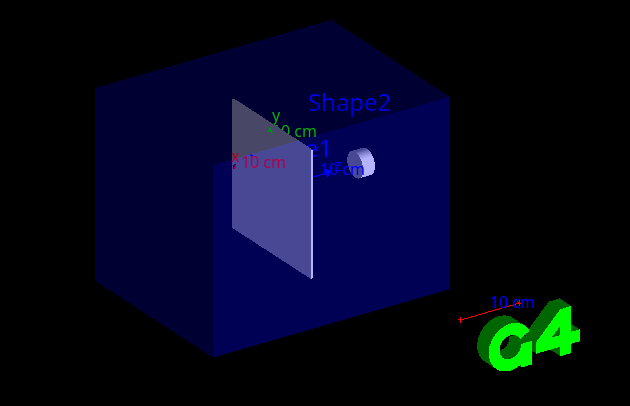
\includegraphics[width=\textwidth,height=0.7\textwidth]{图片4.png}
    \caption{Geant4建模示意图}
    \end{minipage}
    \centering
    \begin{minipage}[t]{0.45\textwidth}
    \centering
    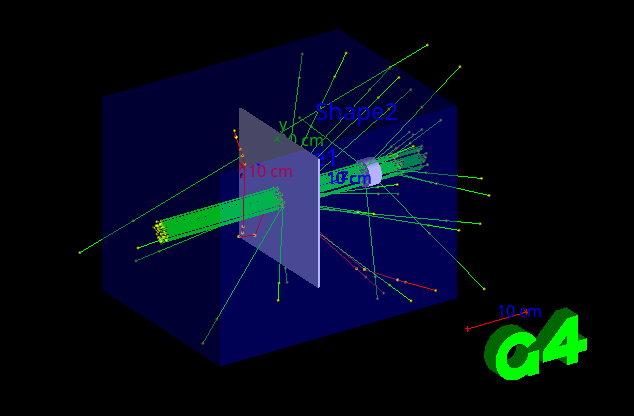
\includegraphics[width=\textwidth,height=0.7\textwidth]{图片5.png}
    \caption{Geant4入射$\gamma$光子示意图}
    \end{minipage}
    \end{figure}
\subsection{模拟计算不同材料材料参数下累积因子}
在验证Geant4模拟结果可信后,在Geant4中选用不同的材料(空气、水、铝、铁、铅、人
体球等)作为屏蔽物质,模拟非准直$\gamma$射线入射实验
根据Geant4所返回的能量沉积结果和注量率等结果,计算对应的累积因子。
\subsection{不同探测距离下的累积因子}
累积因子是由于散射而产生的,因此探测器与屏蔽物质距离的不同
也会导致累积因子的变化。在模拟计算过程中, 选取不同的探测距离,即
不同的$\mu d$值,一般选取光子平均自由程量级
,观察探测器处的能量沉积,根据结果得到累积因子随探测距离的变化。
\subsection{修正无限大介质模型经验公式}
根据模拟实验测得的数据,计算相应累积因子,寻找累积因子的变化规律,
对泰勒公式和伯杰公式进行修正,得到可用于工程实际模型
的累积因子计算经验公式。
\subsection{为伽玛辐射屏蔽材料的选择提供参考}
在前面研究工作的基础上,对屏蔽体进行能量响应的测
试,确定其合适的工作范围,根据不同材料厚度距离下的累积因子,
以及修正过的累积因子计算公式,
综合考虑防护剂量限制及防护成本,
遵照辐射防护三原则,针对实际伽玛辐射的屏蔽材料选择给出合理参考。

\section{进度安排,预期达到的目标}
\begin{table}[htbp]
    \caption{进度安排和预期目标}
    \vspace{0.5em}\centering\wuhao
    \begin{tabular}{ccccc}
    \toprule[1pt]
    时间 & 进度安排\\
    \midrule[2pt]
    12月初-12月末 & 进行Geant4模拟

    与实验及参考值计算结果对比验证\\
    12月末-3月 & 模拟不同条件下的累积因子;撰写中期报告\\
    4月初至5月中旬 & 
    利用模拟结果修正累积因子的经验公式\\
    5月下旬至6月上旬 & 为实际伽玛辐射的屏蔽材料提供参考,
    撰写结题报告\\
    \bottomrule[1.5pt]
    \end{tabular}
    \end{table}
\section{课题已具备和所需的条件、经费}
本课题模拟计算阶段需要计算机与Geant4程序,已经具备。
实验阶段需要的放射源、屏蔽材料以及探测器,核物理实验室已具备,经费充足。
\section{研究过程中可能遇到的困难和问题,解决的措施}
1.实际实验中,不具备探测器一侧的合理准直
装置,受放射源强度限制,也无法进行有效的准直屏蔽。
解决措施:实验目的主要为验证Geant4模拟计算的可靠性,
实际实验中需要准直的部分为无累积因子时的伽马射线衰减,
可采用材料的标准值计算与Geant4模拟验证替代。

2.实际屏蔽材料以及探测器并非理想纯净物,
而Geant4模拟计算内置材料均为理想物质,结果对比可能有偏差。
解决措施:
对于探测器而言,为获得累积因子,需要将沉积能量做比,对最终结果无影响。
对屏蔽材料,可以在Geant4中自定义混合物,进行合理的杂质添加。
\section{主要参考文献}
\bibliographystyle{hithesis}
\bibliography{reference}
% Local Variables:
% TeX-master: "../mainart"
% TeX-engine: xetex
% End: